\documentclass{standalone}
\usepackage{tikz}
\usepackage{pgfplots}
\pgfplotsset{width=32cm,height=18cm,compat=1.3}
\pgfplotsset{every tick label/.append style={font=\Huge}}
\usepackage{filecontents}

\usetikzlibrary{patterns}

\definecolor{citrine}{rgb}{0.89, 0.82, 0.04}

\begin{document}
	\centering
		\vspace{1.5em}
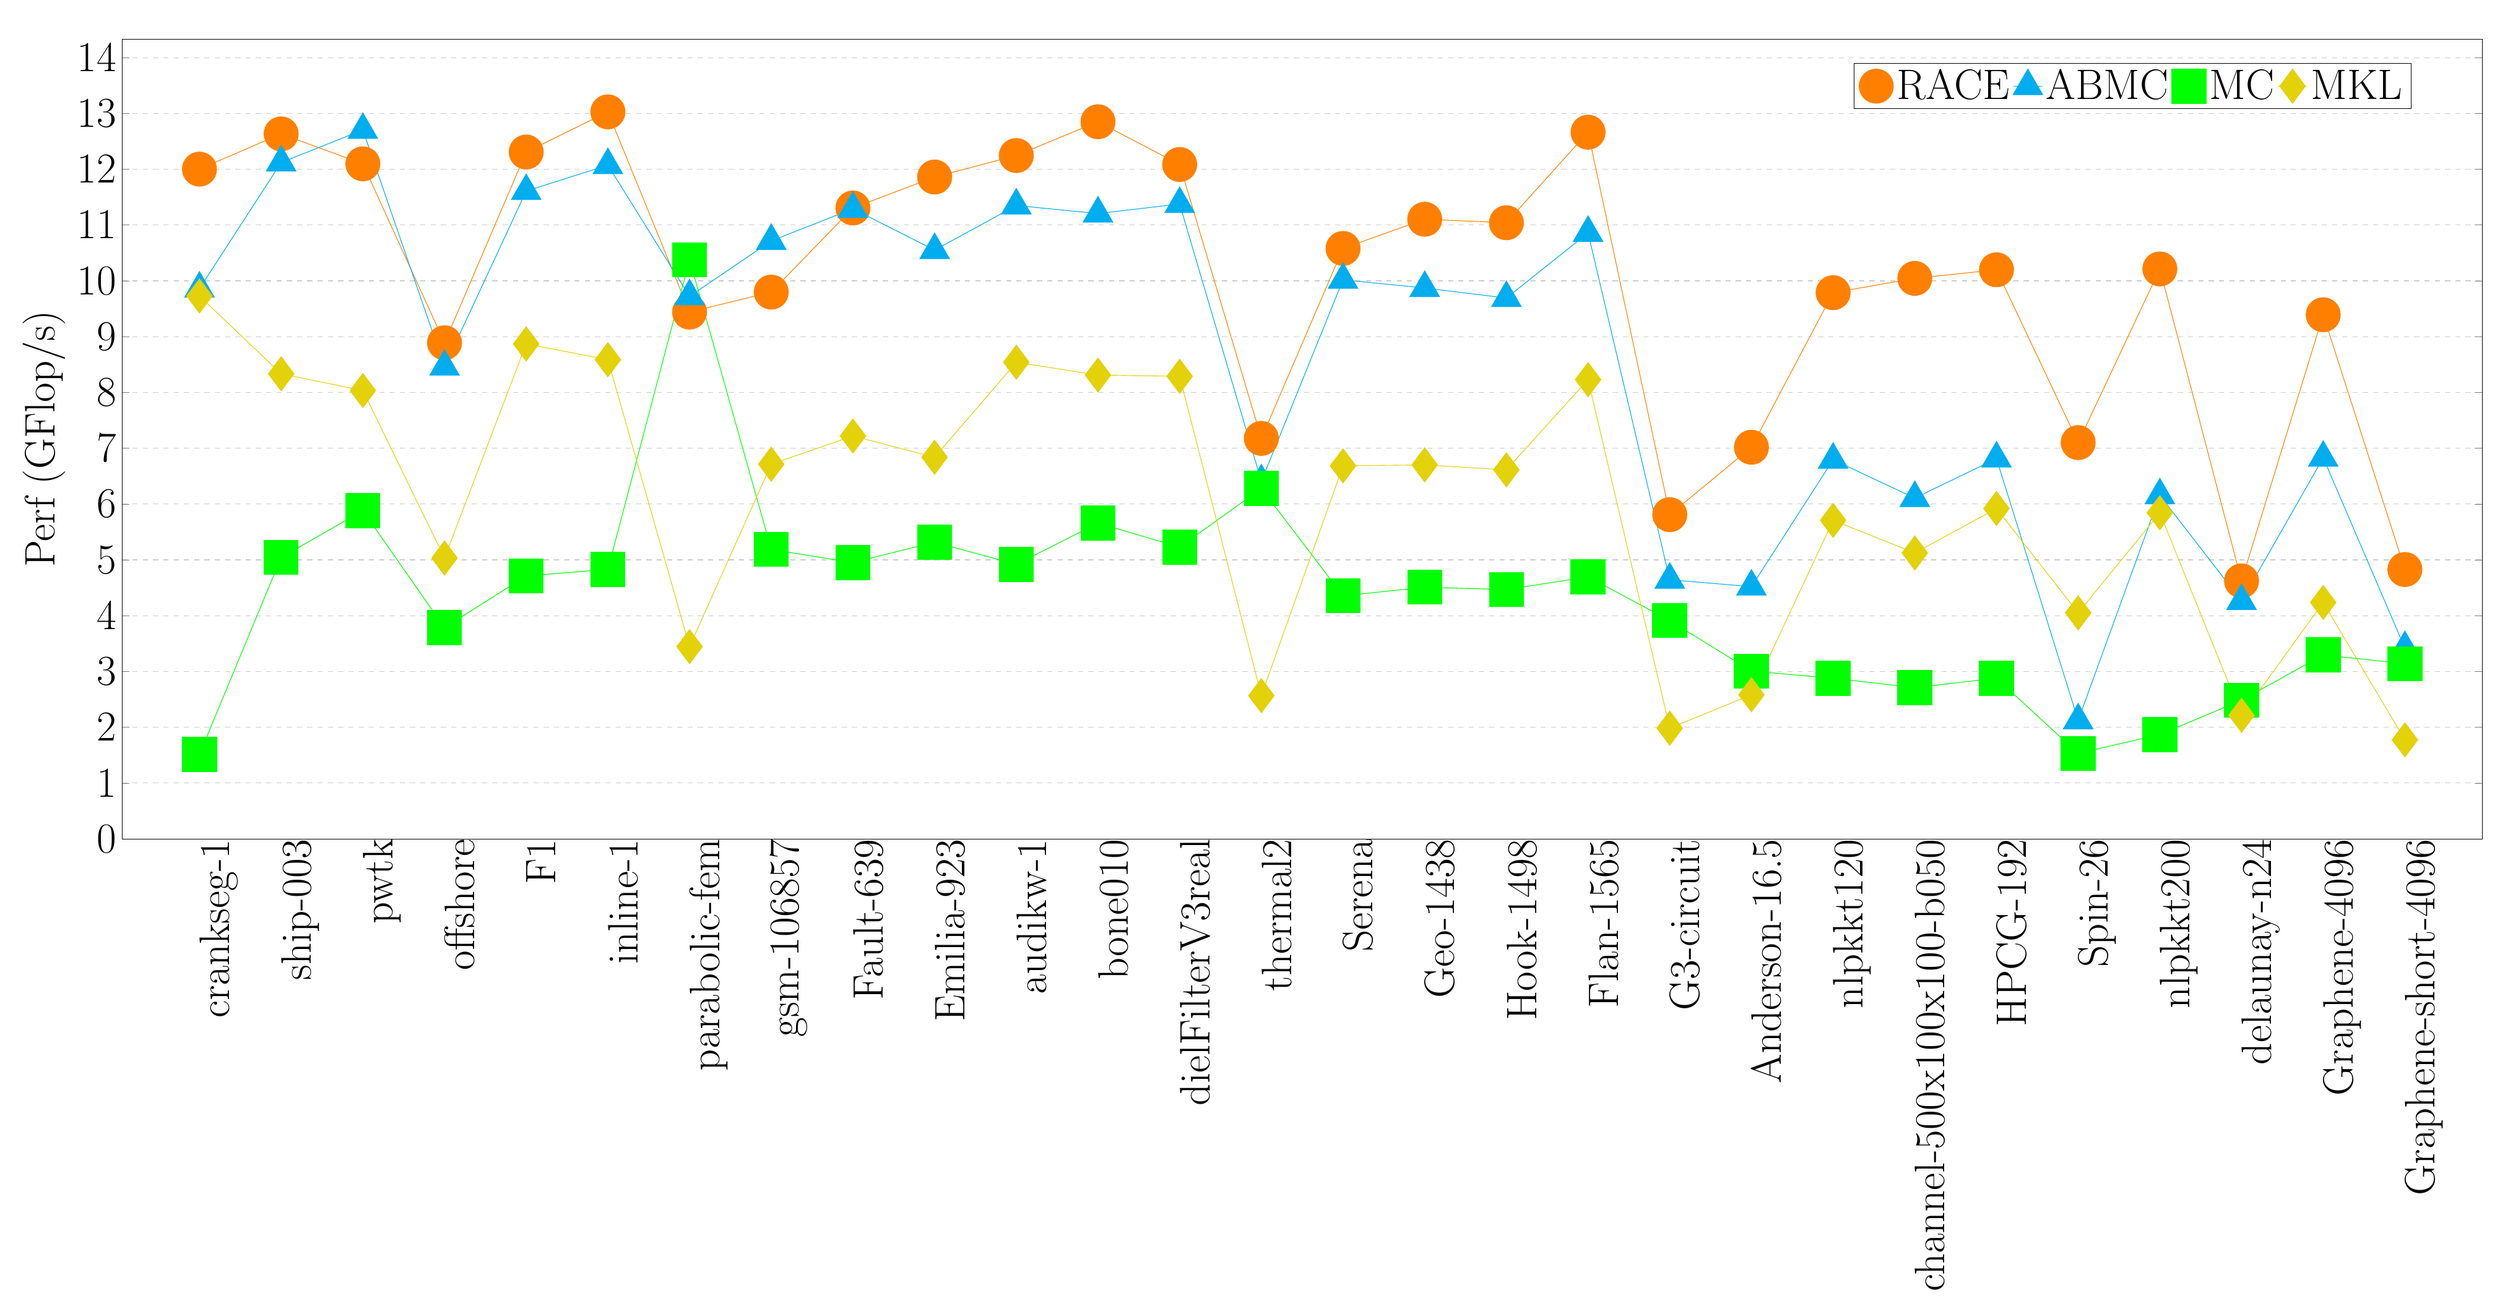
\begin{tikzpicture}
		%	\node at (13.25,15) {\LARGE{}};
			\begin{axis}[
		%	xmin=0.25, xmax=7.25,
			ymin=0, %ymax=3.25,
			xtick={1, 2, 3, 4, 5, 6, 7, 8, 9, 10, 11, 12, 13, 14, 15, 16, 17, 18, 19, 20, 21, 22, 23, 24, 25, 26, 27, 28},
		%	ytick={0,0.5,1,1.5,2,2.5,3},
			xticklabels={crankseg-1, ship-003, pwtk, offshore, F1, inline-1, parabolic-fem, gsm-106857, Fault-639, Emilia-923, audikw-1, bone010, dielFilterV3real, thermal2, Serena, Geo-1438, Hook-1498, Flan-1565, G3-circuit, Anderson-16.5, nlpkkt120, channel-500x100x100-b050, HPCG-192, Spin-26, nlpkkt200, delaunay-n24, Graphene-4096, Graphene-short-4096},
			width  = 50cm,
			height = 18cm,
			major x tick style = transparent,
			%	minor ytick={1, 5, 10, 15, 20, 25, 30 ,35,40},
			grid = minor,	
			%add_bar_commands
			ymajorgrids = true,
			grid style={dashed, gray!40},
			ylabel = {\Huge{Perf (GFlop/s)}},
		%	symbolic x coords={Graphene-2048-2048, Graphene-4096-4096, Spin-24-24-24},
			x tick label style={rotate=90, anchor=north east, inner sep=0mm, font={\Huge}},
			tick label style={font={\Huge}},
			scaled y ticks = false,
			enlarge x limits=0.035,
			legend cell align=left,
			legend style={font=\Huge},
			legend columns=-1,
			legend style={
				%at={(1,1.05)},
				%anchor=south east,
				%column sep=1ex,
				legend pos=north east
			},
			%spl_legend_code
			title= {\Huge\scalebox{1.5}{{}}}
			]

\addplot[mark=*, mark size=10pt, mark options={orange}, draw=orange ] plot coordinates{(1,12.001241) (2,12.632607) (3,12.096590) (4,8.890258) (5,12.308086) (6,13.027954) (7,9.439195) (8,9.797964) (9,11.305451) (10,11.860212) (11,12.245165) (12,12.850634) (13,12.084667) (14,7.176575) (15,10.580104) (16,11.103660) (17,11.040916) (18,12.663604) (19,5.809891) (20,7.017762) (21,9.787395) (22,10.044041) (23,10.198226) (24,7.101122) (25,10.213585) (26,4.623104) (27,9.392370) (28,4.827286)};
\addplot[mark=triangle*, mark size=10pt, mark options={cyan}, draw=cyan ] plot coordinates{(1,9.859968) (2,12.11982) (3,12.703411) (4,8.460706) (5,11.608382) (6,12.072864) (7,9.721248) (8,10.7155) (9,11.290496) (10,10.550108) (11,11.349636) (12,11.205518) (13,11.376125) (14,6.406763) (15,10.017825) (16,9.871436) (17,9.691435) (18,10.858343) (19,4.643185) (20,4.520068) (21,6.793541) (22,6.107278) (23,6.814285) (24,2.123563) (25,6.155564) (26,4.2621) (27,6.828725) (28,3.418198)};
\addplot[mark=square*, mark size=10pt, mark options={green}, draw=green ] plot coordinates{(1,1.515266) (2,5.042036) (3,5.882780) (4,3.785089) (5,4.712229) (6,4.829823) (7,10.379205) (8,5.186203) (9,4.951810) (10,5.315925) (11,4.919472) (12,5.659067) (13,5.228773) (14,6.278711) (15,4.355169) (16,4.509457) (17,4.467384) (18,4.695064) (19,3.912522) (20,3.007262) (21,2.877764) (22,2.711298) (23,2.879436) (24,1.531584) (25,1.869278) (26,2.484245) (27,3.296298) (28,3.139243)};
\addplot[mark=diamond*, mark size=10pt, mark options={citrine}, draw=citrine ] plot coordinates{(1,9.728058) (2,8.333939) (3,8.034666) (4,5.033252) (5,8.870003) (6,8.586093) (7,3.445033) (8,6.714281) (9,7.219080) (10,6.838459) (11,8.540922) (12,8.310591) (13,8.288898) (14,2.566802) (15,6.685272) (16,6.701994) (17,6.612762) (18,8.230405) (19,1.983922) (20,2.582208) (21,5.708207) (22,5.123623) (23,5.920205) (24,4.050526) (25,5.844054) (26,2.214071) (27,4.237317) (28,1.773905)};
	%addplot cmd

	\legend{RACE, ABMC, MC, MKL}

	\end{axis}			
\end{tikzpicture}

\end{document}

